% Options for packages loaded elsewhere
\PassOptionsToPackage{unicode}{hyperref}
\PassOptionsToPackage{hyphens}{url}
%
\documentclass[
]{article}
\usepackage{amsmath,amssymb}
\usepackage{lmodern}
\usepackage{iftex}
\ifPDFTeX
  \usepackage[T1]{fontenc}
  \usepackage[utf8]{inputenc}
  \usepackage{textcomp} % provide euro and other symbols
\else % if luatex or xetex
  \usepackage{unicode-math}
  \defaultfontfeatures{Scale=MatchLowercase}
  \defaultfontfeatures[\rmfamily]{Ligatures=TeX,Scale=1}
\fi
% Use upquote if available, for straight quotes in verbatim environments
\IfFileExists{upquote.sty}{\usepackage{upquote}}{}
\IfFileExists{microtype.sty}{% use microtype if available
  \usepackage[]{microtype}
  \UseMicrotypeSet[protrusion]{basicmath} % disable protrusion for tt fonts
}{}
\makeatletter
\@ifundefined{KOMAClassName}{% if non-KOMA class
  \IfFileExists{parskip.sty}{%
    \usepackage{parskip}
  }{% else
    \setlength{\parindent}{0pt}
    \setlength{\parskip}{6pt plus 2pt minus 1pt}}
}{% if KOMA class
  \KOMAoptions{parskip=half}}
\makeatother
\usepackage{xcolor}
\IfFileExists{xurl.sty}{\usepackage{xurl}}{} % add URL line breaks if available
\IfFileExists{bookmark.sty}{\usepackage{bookmark}}{\usepackage{hyperref}}
\hypersetup{
  pdftitle={12/1/2021 GMAC analysis and pvalue plots},
  pdfauthor={Jarred Kvamme, University of Idaho},
  hidelinks,
  pdfcreator={LaTeX via pandoc}}
\urlstyle{same} % disable monospaced font for URLs
\usepackage[margin=1in]{geometry}
\usepackage{longtable,booktabs,array}
\usepackage{calc} % for calculating minipage widths
% Correct order of tables after \paragraph or \subparagraph
\usepackage{etoolbox}
\makeatletter
\patchcmd\longtable{\par}{\if@noskipsec\mbox{}\fi\par}{}{}
\makeatother
% Allow footnotes in longtable head/foot
\IfFileExists{footnotehyper.sty}{\usepackage{footnotehyper}}{\usepackage{footnote}}
\makesavenoteenv{longtable}
\usepackage{graphicx}
\makeatletter
\def\maxwidth{\ifdim\Gin@nat@width>\linewidth\linewidth\else\Gin@nat@width\fi}
\def\maxheight{\ifdim\Gin@nat@height>\textheight\textheight\else\Gin@nat@height\fi}
\makeatother
% Scale images if necessary, so that they will not overflow the page
% margins by default, and it is still possible to overwrite the defaults
% using explicit options in \includegraphics[width, height, ...]{}
\setkeys{Gin}{width=\maxwidth,height=\maxheight,keepaspectratio}
% Set default figure placement to htbp
\makeatletter
\def\fps@figure{htbp}
\makeatother
\setlength{\emergencystretch}{3em} % prevent overfull lines
\providecommand{\tightlist}{%
  \setlength{\itemsep}{0pt}\setlength{\parskip}{0pt}}
\setcounter{secnumdepth}{-\maxdimen} % remove section numbering
\ifLuaTeX
  \usepackage{selnolig}  % disable illegal ligatures
\fi

\title{12/1/2021 GMAC analysis and pvalue plots}
\author{Jarred Kvamme, University of Idaho}
\date{9/22/2021}

\begin{document}
\maketitle

\section*{1. Overview}

Both MRPC-LOND and MRPC-ADDIS techniques inferred a large number of
trans mediated trios. The trans-mediation model has been previously
identified, but is not the commonly ackowledged mode of mediation. Since
this result is surprising relative to the existing literature, we sought
to apply another method for inferring mediation on a subset of GTEx
trios analyzed herein by MRPC. The Genomic Mediation analysis with
Adaptive Confounding (GMAC) algorithm allows for a unique selection of a
subset of potential confounders, \({\bf X_{ij}}\) from a larger
covariate pool, \({\bf H}\), for each trio. By taking advantage of the
Principle of Mendelian Randomization, the authors filter \({\bf H}\) by
removing common child and intermediate confounding variables (e.g
variables associated with the eQTL as well as the cis/trans genes).
Post-filtering, GMAC preforms a mediation test on the edge between the
cis gene and trans gene via the regression of the trans-gene \(T_j\) on
the cis-eQTL \(L_i\), cis-gene \(C_i\), and the set of adaptively
selected confounders \({\bf X_{ij}}\):

\begin{eqnarray} T_j = \beta_0 + \beta_1 C_i + \beta_2 L_i + {\bf \Gamma} {\bf X}_{ij} + \epsilon \end{eqnarray}

The mediation statistic is the observed \(t\)-value of the cis-gene
coefficient \(\beta_1\). A null distribution for no-mediation is
constructed by iteratively permuting the values of the cis-transcript
within each genotype and repeating the above regression. The authors
argue that the permutation of the cis-transcript within the genotypes of
the cis-eQTL removes the association between the cis and trans gene
transcripts while preserving the higher order associations with the
cis-eQTL. The resulting permutation test for mediation compares the
observed relationship between the trans and cis gene to a null
distribution constructed from a model with no association and assuming
that possible confounding has been well adjusted via the selected
covariates.

It is important to note that the above mediation test describes only the
association between cis-gene and trans-gene transcripts
(\(C_i \leftrightarrow T_j\) ) and does not consider possible effects
between the cis-eQTL and the cis-gene transcript
(\(L_i \rightarrow C_i\)), or the cis-eQTL and trans-gene transcript
(\(L_i \rightarrow T_j\)).

\section*{2. Methods}
\subsection*{2.1 Applying GMAC to GTEx Trios}

To compare the GMAC and MRPC algorithms, we applied the GMAC algorithm
to the top five GTEx tissues by sample size. Following with the creators
of GMAC, we used the full set of principle components retained from the
PCA of the expression matrix as the covariate pool, and three additional
known confounders: the PCR used, the platform used, and sex of the
individual in each sample {[}@yang2017identifying{]}.

Consistent with @yang2017identifying, the analysis was preformed using a
common child and intermediate variable filtering FDR of \(10\%\) and a
confounder selection FDR of \(5\%\) for each trio. Each trio supplied to
GMAC consisted of the cis-QTL and the PEER normalized cis and trans gene
transcripts with the highest association to the eQTL. To mitigate
missing values in the eQTL matrix, multiple imputation of the matrix of
unique cis-eQTLs was preformed via multiple correspondence analysis
(MCA) prior to its use in GMAC {[}@josse2016missmda{]}. The analysis was
preformed twice on each trio, first with the cis gene as the mediator
and second with the trans gene as the mediator. This allowed for GMAC
inferred trios to be decomposed into the three groupings used under
MRPC: 1) Cis-gene mediation, 2) Trans-gene mediation, 3) both
(undirected).

\subsection*{2.2 Comparison of GMAC and MRPC Results}

After applying GMAC to each tissue, the false discovery rate among the
retained mediation p-values was controlled at the more liberal rate of
\(10\%\) {[}@yang2017identifying{]}. Each trio determined to have
significant mediation after FDR filtering was compared with the
regulatory network type inferred by MRPC-ADDIS. MRPC-ADDIS can infer
three types of regulatory networks that contain an edge between the cis
and trans gene (M1, M2, or M4). Since GMAC considers only the presence
of the edge and not its direction, trios inferred to be one of M1, M2,
or M4 under ADDIS, that were also significant under GMAC, were
considered consistent (e.g \(C_i \rightarrow T_j\);
\(T_j \rightarrow C_i\); \(C_i \leftrightarrow T_j\) are synonymous
under GMAC).

\subsection*{2.3 Simulations}

\indent \(\bullet\) The Small True Model Simulation (STM)

To further understand the conflict in edge determination between
MRPC-ADDIS and GMAC, we simulated the mediation test - the test for the
\(\beta_1\) coefficient in the presence of all adaptively selected
confounders, \({\bf X}_{ij}\), as described by the regression in
\textbf{eq (1)} - under two different scenarios. (i) To observe the
predictive power of the mediation test when the trans gene comes from a
set of explanatory variables smaller than those in \({\bf X}_{ij}\), We
simulated the trans gene of each trio using the linear relationship:

\begin{eqnarray} T^{\ast}_{j} = \hat{\beta_0}+\hat{\beta_1}C_i + \hat{\beta_2}L_i + \hat{{\bf\Gamma}}_W {\bf W}_{ij} +\epsilon  \end{eqnarray}

where \(T^{\ast}_{j}\) is the simulated trans gene, the coefficients are
replaced by their estimates from the regression in \textbf{eq (1)}, the
errors are \(\epsilon \sim N(0, \hat{\sigma})\), and \({\bf W}_{ij}\) is
a subset of confounders in \({\bf X}_{ij}\) representing the ``highly''
significant confounders from \textbf{eq (1)} (\(p<0.001\)). Note that if
the GMAC inferred mediation type was trans gene mediation only then the
cis gene was simulated and the mediation test was preformed on the
\(\beta_1\) coefficient from regression of the cis gene:
\(C_i = \beta_0 + \beta_1T_j + \beta_2L_i + {\bf \Gamma X}_{ij}+\epsilon\).

We refer to the trans-gene generating function in \textbf{(2)} as the
Small True Model (STM) as the simulated trans gene comes from a model
that is a subset of the explanatory variables in the analysis model
described in \textbf{(1)}. The simulated mediation test then replaces
\(T_j\) in \textbf{(1)} with the simulated trans gene \(T^{\ast}_j\).
Therefore, the simulated mediation test under the STM can be decomposed
as the test on the \(\beta_1\) coefficient obtained from the regression:

\begin{eqnarray} T^{\ast}_{j} = \beta_0+\beta_1C_i + \beta_2L_i + {\bf\Gamma}_{1,W} {\bf W}_{ij} + {\bf \Gamma}_{2,M}{\bf M}_{ij} +\epsilon \end{eqnarray}

where \({\bf M}_{ij}\) represents the additional confounders in
\({\bf X}_{ij}\) that are not included in \({\bf W}_{ij}\) see
\textbf{Figure 1}.

\indent \(\bullet\) The Large True Model Simulation (LTM)

Conversely, a second simulation model was implemented to observe the
power of the mediation test when the generating model for the trans gene
is larger than the model used to infer the mediation relationship. In
this scenario, the trans gene is simulated via:

\begin{eqnarray} T^{\ast}_{j} = \hat{\beta}_0+\hat{\beta}_1C_i + \hat{\beta}_2L_i + \hat{{\bf \Gamma}}_V{\bf V}_{ij} +\epsilon  \end{eqnarray}

which we refer to as the Large True Model (LTM). Note that the
coefficient estimates in \textbf{(4)} come from the regression of the
original data on a larger set than in \textbf{eq. (1)}:

\begin{eqnarray} T_{j} = \beta_0+\beta_1C_i + \beta_2L_i + {\bf\Gamma} {\bf X}_{ij} + {\bf \Gamma}_{G}{\bf G}_{ij} +\epsilon \end{eqnarray}

where \({\bf G}_{ij}\) represents the additional explanatory variables
in \({\bf V}_{ij}\) not in \({\bf X}_{ij}\) (see \textbf{Figure 1}). The
additional variables represented by \({\bf G}_{ij}\) were randomly
selected from the confounder pool \({\bf H}\) with equal probability.
The four sets of \(p\)-values (GMAC mediation \(p\)-value, GMAC
permutation \(p\)-value, the STM mediation \(p\)-value, and the LTM
mediation \(p\)-value) were visually inspected to determine the effect
of model mis-specification on the power of the mediation and permutation
test(s).

\indent \(\bullet\) True GMAC Model Simulation (TGM)

We preformed a third simulation of the trans gene using the analysis
model in GMAC given by \textbf{(1)} as the trans gene generating
process. We then applied the MRPC model

\begin{eqnarray}  T_j = \beta_0 + \beta_1 C_i +\beta_2 L_i + {\bf \Gamma}_z {\bf Z}_{ij} \end{eqnarray}

where the column dimension \({\bf Z}_{ij}\) is a less than or equal to
the column dimension of \({W}_{ij}\) and represents only the confounders
selected under the MRPC PC-selection methodology. The goal was to
analyze the power of MRPC in detecting the mediation edge when the data
is generated from the much larger GMAC model.

\indent \(\bullet\) GMAC Self Simulation (GSS)

We created a fourth simulation scenario to test the importance of
permutation on the analysis result. Each of the above simulations seeks
to understanding the inferential power of MRPC/GMAC under model
misspecification. In this scenario we take a different approach and use
the model suggested by GMAC for each trio given by \textbf{eqn. (1)} to
generate the trans gene such that:

\[ T_j^{\ast} = \hat{\beta}_0 + \hat{\beta}_1 C_i + \hat{\beta}_2 L_i + \hat{{\bf \Gamma}} {\bf X}_{ij} + \epsilon  \]

where \(\epsilon \sim N(0, \hat{\sigma})\). We then apply the correct
model \({\bf (1)}\) to each simulated trio under this scenario to obtain
the parametric and permutation inferences when we know the analysis
model is correct.

\section*{3. Results}
\subsection*{3.1 Comparing GMAC and MRPC}

In light of the surprising number of trans-gene mediation trios inferred
by MRPC, we sought to compare our results with GMAC by applying the GMAC
method to the top five GTEx tissues by sample size. It is important to
note that the test for mediation used by GMAC describes only the
association between cis-gene and trans-gene transcripts
(\(C_i \leftrightarrow T_j\) ) and does not consider the possible
effects between the cis-eQTL and the cis-gene (\(L_i \rightarrow C_i\)),
or the cis-eQTL and trans-gene (\(L_i \rightarrow T_j\)). Therefore,
since GMAC considers only the presence of the mediation edge, trios
inferred to be one of M1, M2, or M4 under ADDIS, that were also
significant under GMAC, were considered consistent (e.g
\(C_i \rightarrow T_j\); \(T_j \rightarrow C_i\);
\(C_i \leftrightarrow T_j\) are synonymous under GMAC).

At the \(10\%\) false discovery rate, GMAC identified \(2,160\) trios
with an edge between the cis and trans genes out of \(55,446\) total
trios tested across the five selected tissues: Adipose subcutaneous,
Tibial artery, Muscle skeletal, Sun exposed skin, and Whole blood. Of
the trios with mediation edges, 653 were identified as the cis gene
mediating the trans gene, 245 as trans gene mediating the cis gene and
1,345 as both (\(29.1\%, 10.9\%\), and \(60\%\) respectively). As can be
seen from \textbf{Table 2}, the consistency in inferred mediation edges
between the two methods varied between \(39\%\) and \(50\%\) of the
trios across tissues.

\subsection*{3.2 Simulation Results}

\(\bullet\) - We noticed that the mediation parametric p-value can vary
quite a bit. we ran each simulation scenario 1000 times on each trio and
obtained the median p-value from each of the 4 scenarios. We used this
as a robust estimate of the parametric p-value

\(\bullet\) - The nominal p-value and mediation p-value give more or
less the same value except for rare variant trios

\(\bullet\) - We noticed that Badsha implemented the PC selection code
for MRPC in a way that led to the qvalues of each correlation test being
applied after the p-values had already been bonferroni adjusted. This
lead to extremely few PCs being selected for each trio. After
implementing the correct PC selection process, MRPC and GMAC select
equivalent numbers of PCs

\(\bullet\) - Figure 1 panel D supports that the nominal p-value appears
to be better at determining the presence of a mediation edge for rare
variants. This indicates we may need to preform the permuted regression
test when the instrumental variable/ cis-eQTL contains a rare allele

\(\bullet\) - Figure 1 panels A-C supports the need to skip the marginal
tests and instead proceed directly to the conditional tests for each
edge. However, these plots do not consider the entire model topology
only the presence or absence of the mediation edge: \(T_1 - T_2\)

\newpage
\section{Tables and Figures}

\begin{longtable}[]{@{}
  >{\raggedright\arraybackslash}p{(\columnwidth - 10\tabcolsep) * \real{0.0909}}
  >{\raggedleft\arraybackslash}p{(\columnwidth - 10\tabcolsep) * \real{0.2386}}
  >{\raggedleft\arraybackslash}p{(\columnwidth - 10\tabcolsep) * \real{0.1591}}
  >{\raggedleft\arraybackslash}p{(\columnwidth - 10\tabcolsep) * \real{0.1818}}
  >{\raggedleft\arraybackslash}p{(\columnwidth - 10\tabcolsep) * \real{0.1932}}
  >{\raggedleft\arraybackslash}p{(\columnwidth - 10\tabcolsep) * \real{0.1364}}@{}}
\caption{Descriptive statistics for the distribution of missing values
across the eQTL's for each tissue used in GMAC}\tabularnewline
\toprule
\begin{minipage}[b]{\linewidth}\raggedright
\end{minipage} & \begin{minipage}[b]{\linewidth}\raggedleft
Adipose Subcutaneous
\end{minipage} & \begin{minipage}[b]{\linewidth}\raggedleft
Artery Tibial
\end{minipage} & \begin{minipage}[b]{\linewidth}\raggedleft
Muscle Skeletal
\end{minipage} & \begin{minipage}[b]{\linewidth}\raggedleft
Skin Sun Exposed
\end{minipage} & \begin{minipage}[b]{\linewidth}\raggedleft
Whole Blood
\end{minipage} \\
\midrule
\endfirsthead
\toprule
\begin{minipage}[b]{\linewidth}\raggedright
\end{minipage} & \begin{minipage}[b]{\linewidth}\raggedleft
Adipose Subcutaneous
\end{minipage} & \begin{minipage}[b]{\linewidth}\raggedleft
Artery Tibial
\end{minipage} & \begin{minipage}[b]{\linewidth}\raggedleft
Muscle Skeletal
\end{minipage} & \begin{minipage}[b]{\linewidth}\raggedleft
Skin Sun Exposed
\end{minipage} & \begin{minipage}[b]{\linewidth}\raggedleft
Whole Blood
\end{minipage} \\
\midrule
\endhead
Min. & 0.000000 & 0.000000 & 0.000000 & 0.000000 & 0.000000 \\
1st Qu. & 0.000000 & 0.000000 & 0.000000 & 0.000000 & 0.000000 \\
Median & 0.000000 & 0.000000 & 0.000000 & 0.000000 & 0.000000 \\
Mean & 0.006365 & 0.006625 & 0.006560 & 0.006701 & 0.006103 \\
3rd Qu. & 0.003442 & 0.003425 & 0.002833 & 0.003306 & 0.002985 \\
Max. & 0.156627 & 0.159247 & 0.158640 & 0.160331 & 0.155224 \\
\bottomrule
\end{longtable}

\begin{longtable}[]{@{}
  >{\raggedright\arraybackslash}p{(\columnwidth - 16\tabcolsep) * \real{0.2353}}
  >{\raggedleft\arraybackslash}p{(\columnwidth - 16\tabcolsep) * \real{0.0471}}
  >{\raggedleft\arraybackslash}p{(\columnwidth - 16\tabcolsep) * \real{0.0353}}
  >{\raggedleft\arraybackslash}p{(\columnwidth - 16\tabcolsep) * \real{0.0353}}
  >{\raggedleft\arraybackslash}p{(\columnwidth - 16\tabcolsep) * \real{0.0471}}
  >{\raggedleft\arraybackslash}p{(\columnwidth - 16\tabcolsep) * \real{0.0471}}
  >{\raggedleft\arraybackslash}p{(\columnwidth - 16\tabcolsep) * \real{0.0706}}
  >{\raggedleft\arraybackslash}p{(\columnwidth - 16\tabcolsep) * \real{0.2353}}
  >{\raggedleft\arraybackslash}p{(\columnwidth - 16\tabcolsep) * \real{0.2471}}@{}}
\caption{The breakdown of unqiue trios with inferred significant cis or
trans mediation under GMAC across their respective ADDIS inferred
regulatory networks. The column ``Percentage In Common'' is the
proportion of significant trios that also contained a mediation edge in
the regulatory network inferred under ADDIS}\tabularnewline
\toprule
\begin{minipage}[b]{\linewidth}\raggedright
Tissue
\end{minipage} & \begin{minipage}[b]{\linewidth}\raggedleft
M0
\end{minipage} & \begin{minipage}[b]{\linewidth}\raggedleft
M1
\end{minipage} & \begin{minipage}[b]{\linewidth}\raggedleft
M2
\end{minipage} & \begin{minipage}[b]{\linewidth}\raggedleft
M3
\end{minipage} & \begin{minipage}[b]{\linewidth}\raggedleft
M4
\end{minipage} & \begin{minipage}[b]{\linewidth}\raggedleft
Other
\end{minipage} & \begin{minipage}[b]{\linewidth}\raggedleft
Total GMAC Inferred
\end{minipage} & \begin{minipage}[b]{\linewidth}\raggedleft
Percentage In Common
\end{minipage} \\
\midrule
\endfirsthead
\toprule
\begin{minipage}[b]{\linewidth}\raggedright
Tissue
\end{minipage} & \begin{minipage}[b]{\linewidth}\raggedleft
M0
\end{minipage} & \begin{minipage}[b]{\linewidth}\raggedleft
M1
\end{minipage} & \begin{minipage}[b]{\linewidth}\raggedleft
M2
\end{minipage} & \begin{minipage}[b]{\linewidth}\raggedleft
M3
\end{minipage} & \begin{minipage}[b]{\linewidth}\raggedleft
M4
\end{minipage} & \begin{minipage}[b]{\linewidth}\raggedleft
Other
\end{minipage} & \begin{minipage}[b]{\linewidth}\raggedleft
Total GMAC Inferred
\end{minipage} & \begin{minipage}[b]{\linewidth}\raggedleft
Percentage In Common
\end{minipage} \\
\midrule
\endhead
AdiposeSubcutaneous & 107 & 47 & 12 & 102 & 134 & 2 & 404 & 0.4777 \\
ArteryTibial & 88 & 37 & 10 & 108 & 112 & 0 & 355 & 0.4479 \\
MuscleSkeletal & 126 & 37 & 8 & 145 & 132 & 2 & 450 & 0.3933 \\
SkinSunExposed & 118 & 42 & 12 & 132 & 139 & 0 & 443 & 0.4357 \\
WholeBlood & 107 & 55 & 29 & 142 & 171 & 4 & 508 & 0.5020 \\
\bottomrule
\end{longtable}

\begin{longtable}[]{@{}
  >{\raggedright\arraybackslash}p{(\columnwidth - 16\tabcolsep) * \real{0.1370}}
  >{\raggedleft\arraybackslash}p{(\columnwidth - 16\tabcolsep) * \real{0.0822}}
  >{\raggedleft\arraybackslash}p{(\columnwidth - 16\tabcolsep) * \real{0.0890}}
  >{\raggedleft\arraybackslash}p{(\columnwidth - 16\tabcolsep) * \real{0.1712}}
  >{\raggedleft\arraybackslash}p{(\columnwidth - 16\tabcolsep) * \real{0.1849}}
  >{\raggedleft\arraybackslash}p{(\columnwidth - 16\tabcolsep) * \real{0.0753}}
  >{\raggedleft\arraybackslash}p{(\columnwidth - 16\tabcolsep) * \real{0.0890}}
  >{\raggedleft\arraybackslash}p{(\columnwidth - 16\tabcolsep) * \real{0.0822}}
  >{\raggedleft\arraybackslash}p{(\columnwidth - 16\tabcolsep) * \real{0.0890}}@{}}
\caption{Breakdown of trios with inferred mediation under GMAC across
both cis and trans mediation types. The column ``Unique Both''
represents the intersection of the columns ``Total Cis Mediated'' and
``Total Trans Mediated''}\tabularnewline
\toprule
\begin{minipage}[b]{\linewidth}\raggedright
Tissue
\end{minipage} & \begin{minipage}[b]{\linewidth}\raggedleft
Sample Size
\end{minipage} & \begin{minipage}[b]{\linewidth}\raggedleft
Tested Trios
\end{minipage} & \begin{minipage}[b]{\linewidth}\raggedleft
Cis-Gene Mediation Trios
\end{minipage} & \begin{minipage}[b]{\linewidth}\raggedleft
Trans-Gene Mediation Trios
\end{minipage} & \begin{minipage}[b]{\linewidth}\raggedleft
Unique Cis
\end{minipage} & \begin{minipage}[b]{\linewidth}\raggedleft
Unique Trans
\end{minipage} & \begin{minipage}[b]{\linewidth}\raggedleft
Unique Both
\end{minipage} & \begin{minipage}[b]{\linewidth}\raggedleft
Unique Total
\end{minipage} \\
\midrule
\endfirsthead
\toprule
\begin{minipage}[b]{\linewidth}\raggedright
Tissue
\end{minipage} & \begin{minipage}[b]{\linewidth}\raggedleft
Sample Size
\end{minipage} & \begin{minipage}[b]{\linewidth}\raggedleft
Tested Trios
\end{minipage} & \begin{minipage}[b]{\linewidth}\raggedleft
Cis-Gene Mediation Trios
\end{minipage} & \begin{minipage}[b]{\linewidth}\raggedleft
Trans-Gene Mediation Trios
\end{minipage} & \begin{minipage}[b]{\linewidth}\raggedleft
Unique Cis
\end{minipage} & \begin{minipage}[b]{\linewidth}\raggedleft
Unique Trans
\end{minipage} & \begin{minipage}[b]{\linewidth}\raggedleft
Unique Both
\end{minipage} & \begin{minipage}[b]{\linewidth}\raggedleft
Unique Total
\end{minipage} \\
\midrule
\endhead
AdiposeSubcutaneous & 581 & 11850 & 374 & 282 & 122 & 30 & 252 & 404 \\
ArteryTibial & 584 & 11471 & 334 & 226 & 129 & 21 & 205 & 355 \\
MuscleSkeletal & 706 & 10257 & 401 & 314 & 136 & 49 & 265 & 450 \\
SunExposedSkin & 605 & 13045 & 404 & 333 & 110 & 39 & 294 & 443 \\
WholeBlood & 670 & 8823 & 451 & 398 & 110 & 57 & 341 & 508 \\
\bottomrule
\end{longtable}

\begin{figure}
\centering
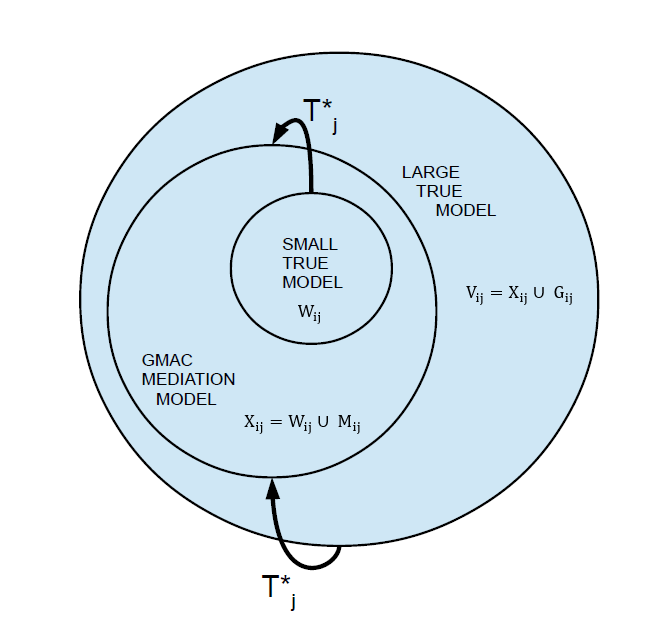
\includegraphics{C:/Users/Bruin/Documents/GitHub/MRPC_support/Manuscript/GMACwriteup_sim_diagram.png}
\caption{A visual depiction of the relationship between the STM and LTM
simulation models for the trans gene and the regression used for the
mediation test}
\end{figure}

\hypertarget{variance-across-tissues-plots}{%
\subsection{variance across tissues
plots}\label{variance-across-tissues-plots}}

\begin{figure}
\centering
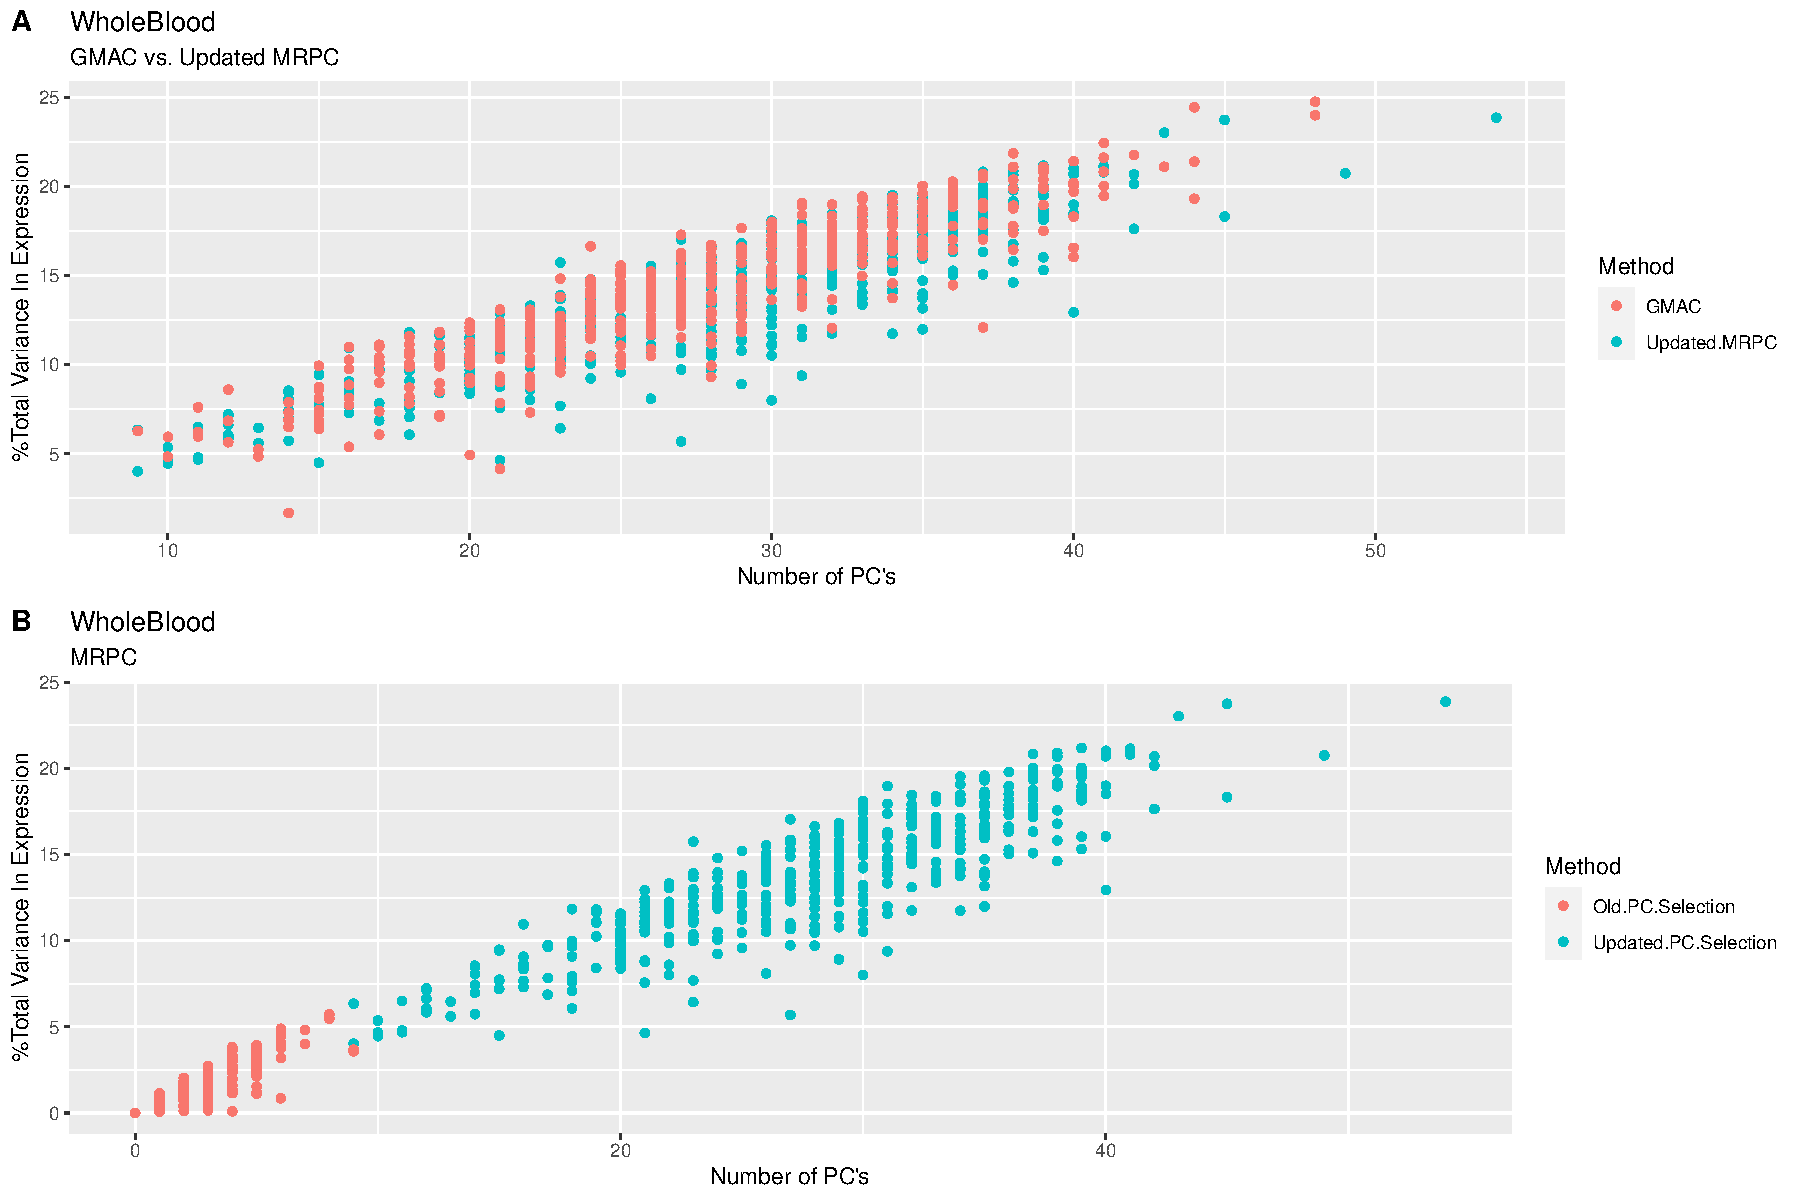
\includegraphics{12_15_2021_GMAC_plots_all_trios_files/figure-latex/unnamed-chunk-4-1.pdf}
\caption{A) The number of PC's included for each trio in whole blood
after using the corrected PC selection for MRPC with the number of PC's
selected by GMAC. B) compares the number of PC's selected for each trio
under Badsha's original code vs the corrected version of PC selection}
\end{figure}

\hypertarget{simulations-median-p-value-plots}{%
\subsection{simulation(s) Median P-value
plots}\label{simulations-median-p-value-plots}}

\begin{figure}
\centering
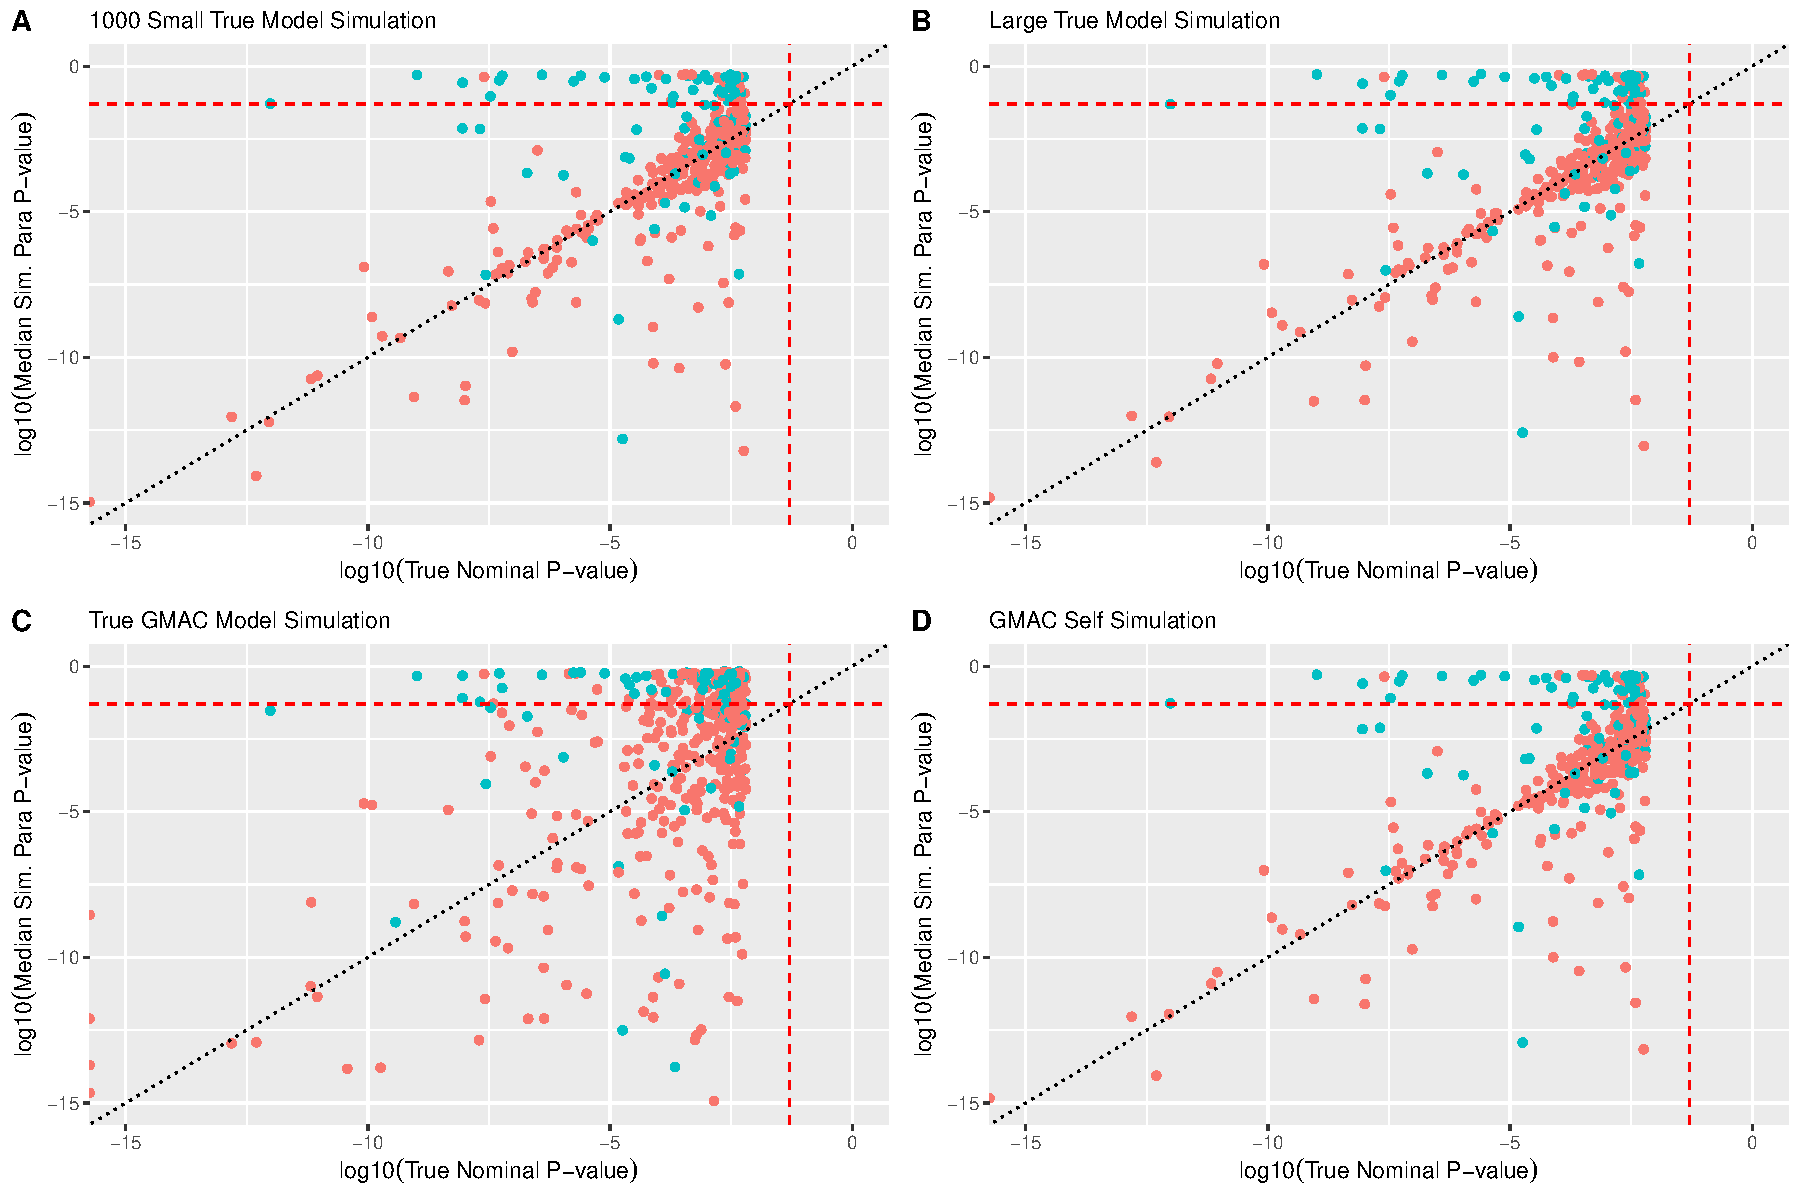
\includegraphics{12_15_2021_GMAC_plots_all_trios_files/figure-latex/unnamed-chunk-5-1.pdf}
\caption{All panels: comparison of the median \(p\)-value from the test
for the mediation edge from 1000 iterations of each simulation scenario
for each trio (y-axis) with the nominal p-value for the edge from the
true model (x-axis). Each panel corresponds to a specific simulation
scenario. These graphs support the need to use conditional tests
directly as well as the need for the permutation test when the genotype
has a low frequency allele.}
\end{figure}

\hypertarget{simulations-nominal-p-value-plots}{%
\subsection{simulation(s) Nominal P-value
plots}\label{simulations-nominal-p-value-plots}}

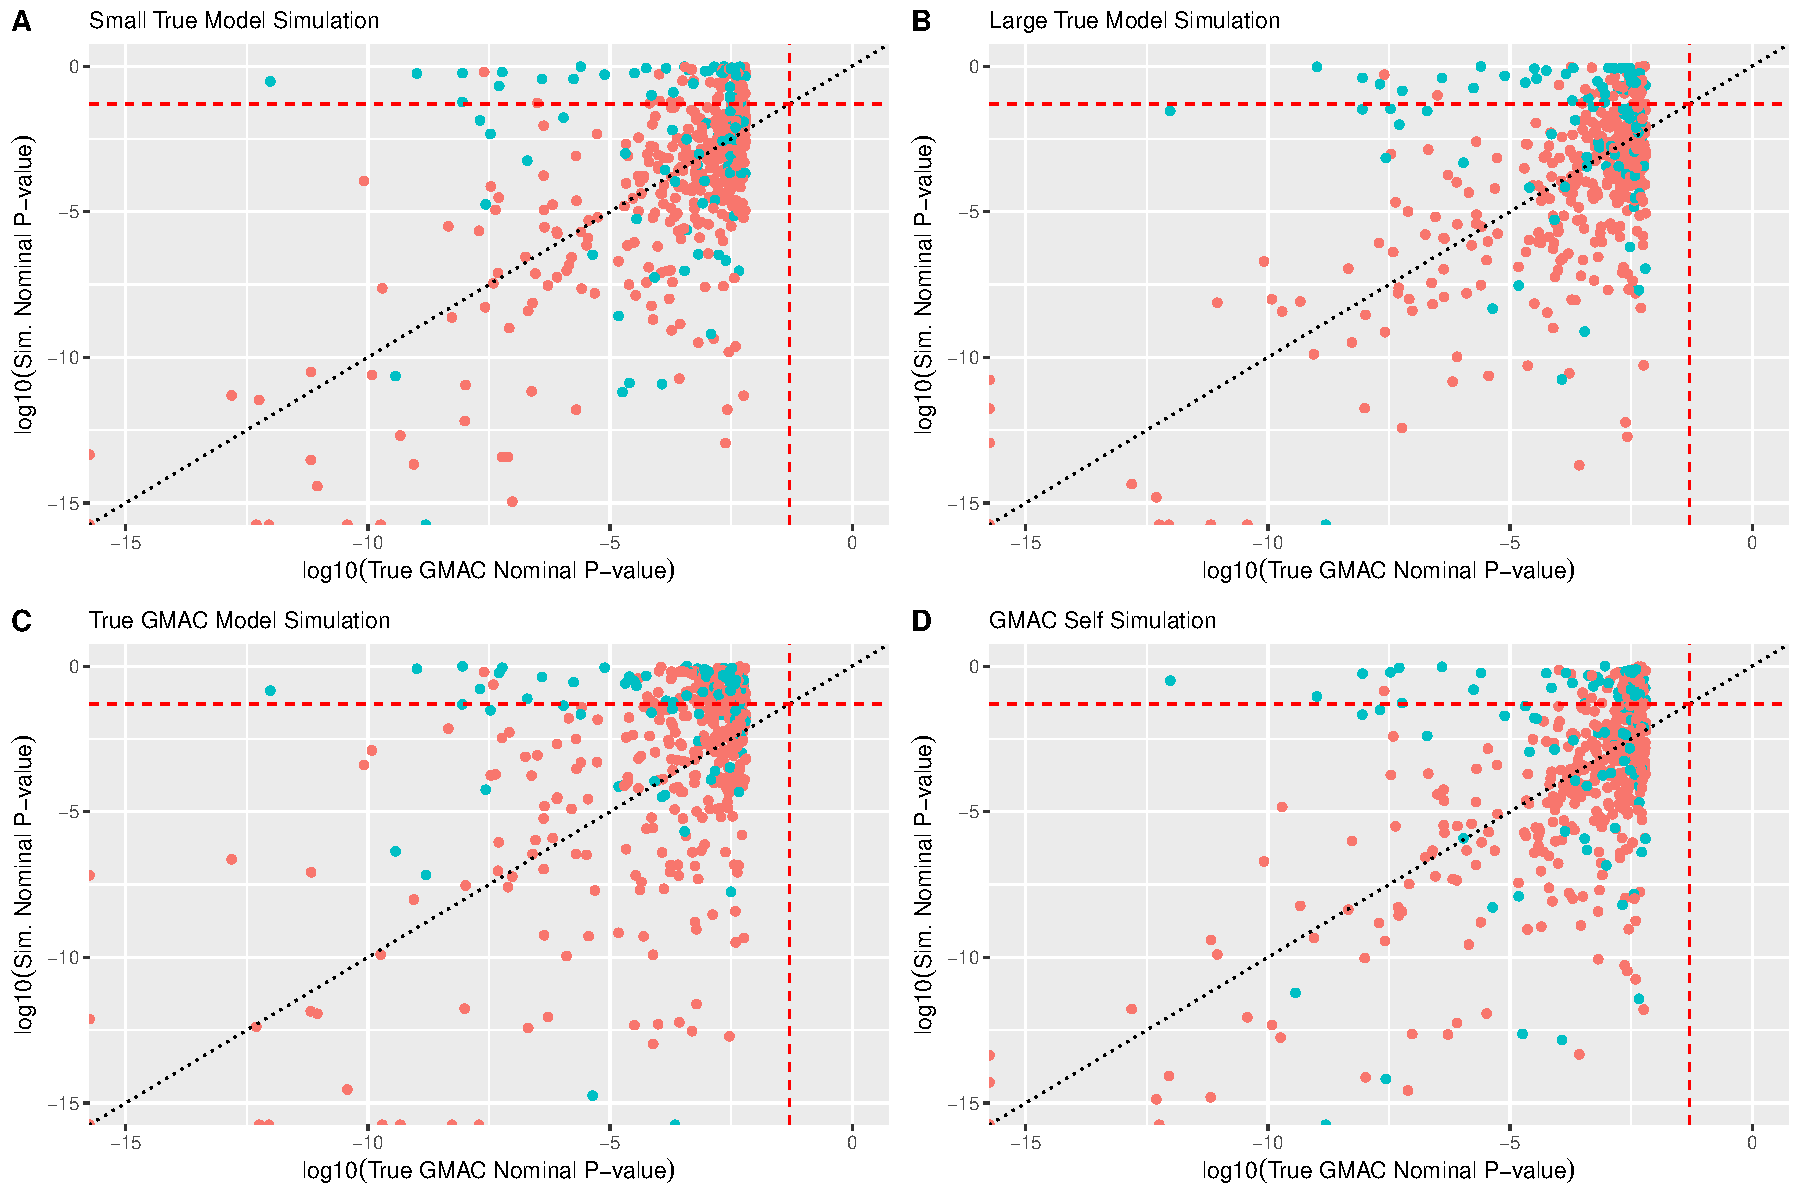
\includegraphics{12_15_2021_GMAC_plots_all_trios_files/figure-latex/unnamed-chunk-6-1.pdf}

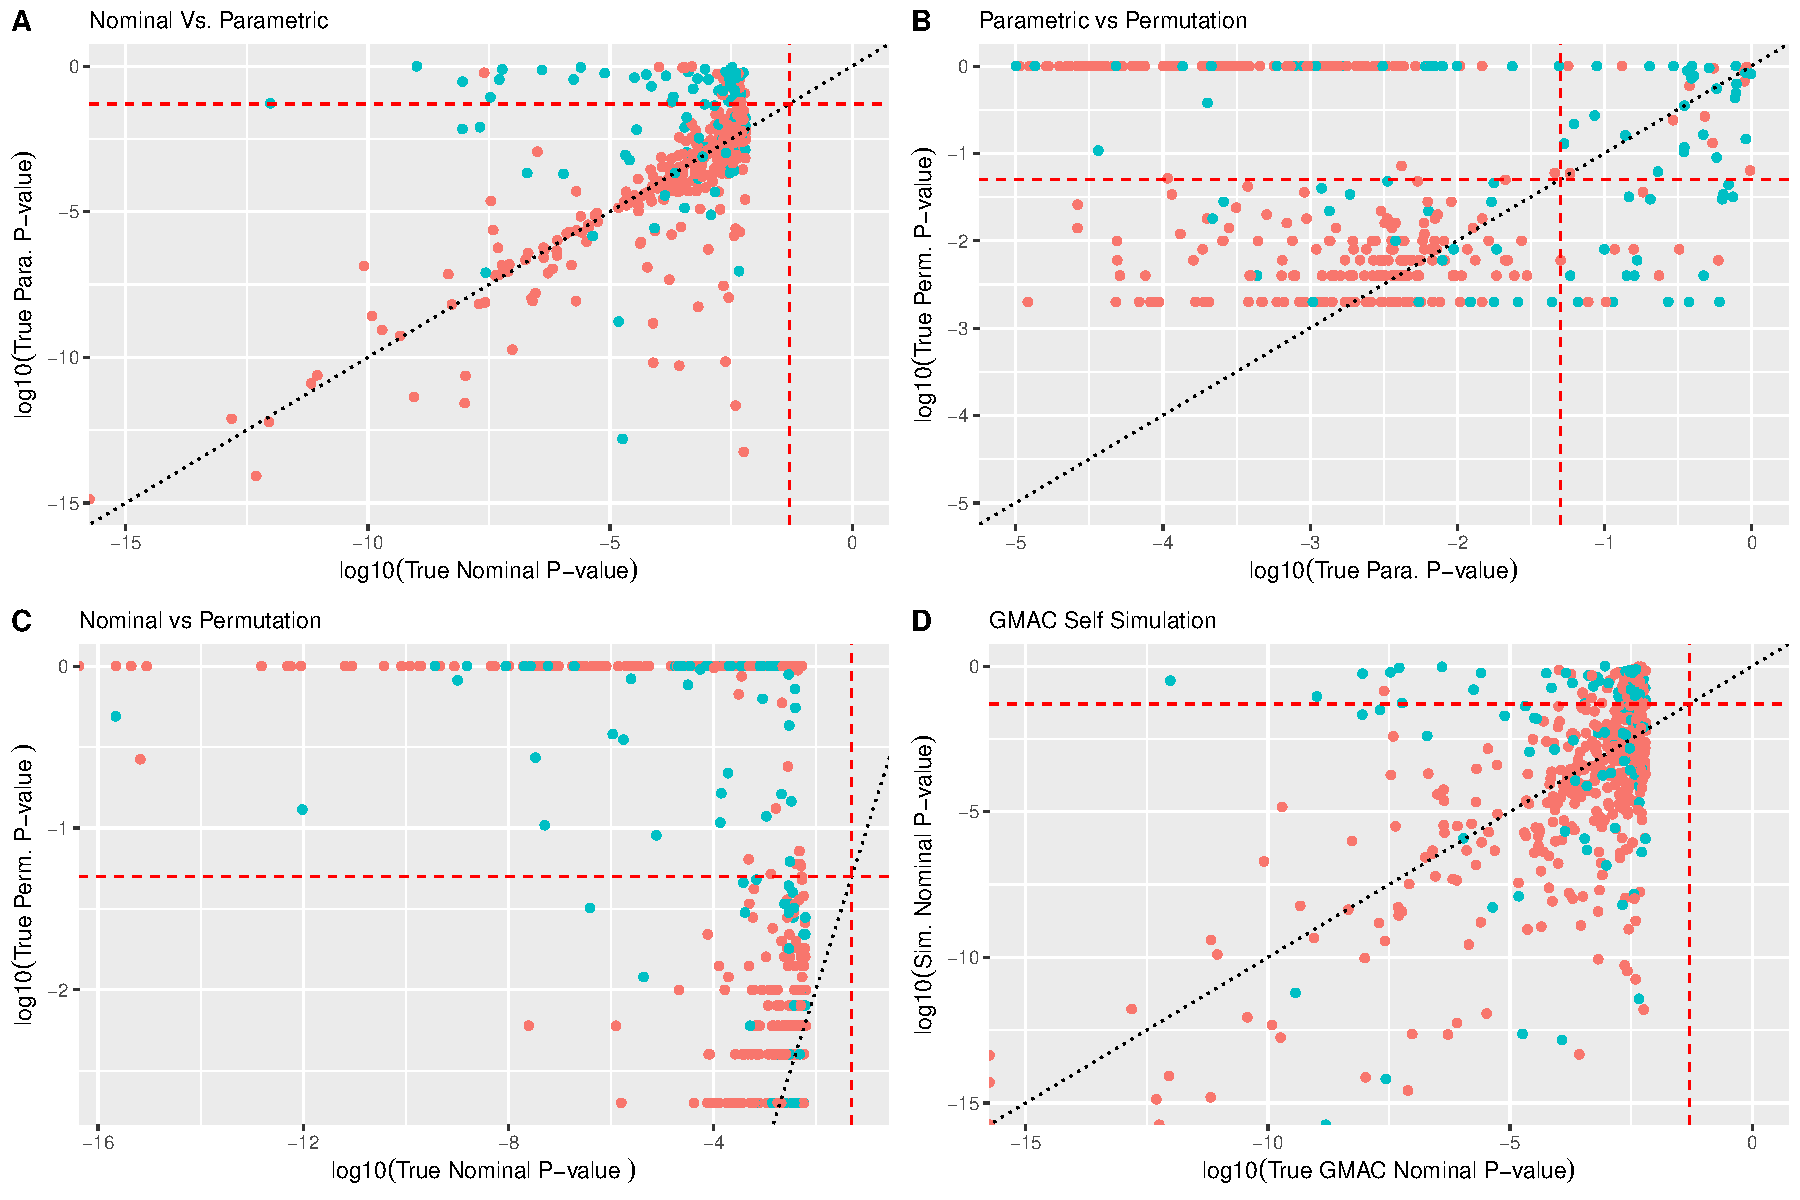
\includegraphics{12_15_2021_GMAC_plots_all_trios_files/figure-latex/unnamed-chunk-7-1.pdf}

\(\bullet\) Rare allele plots

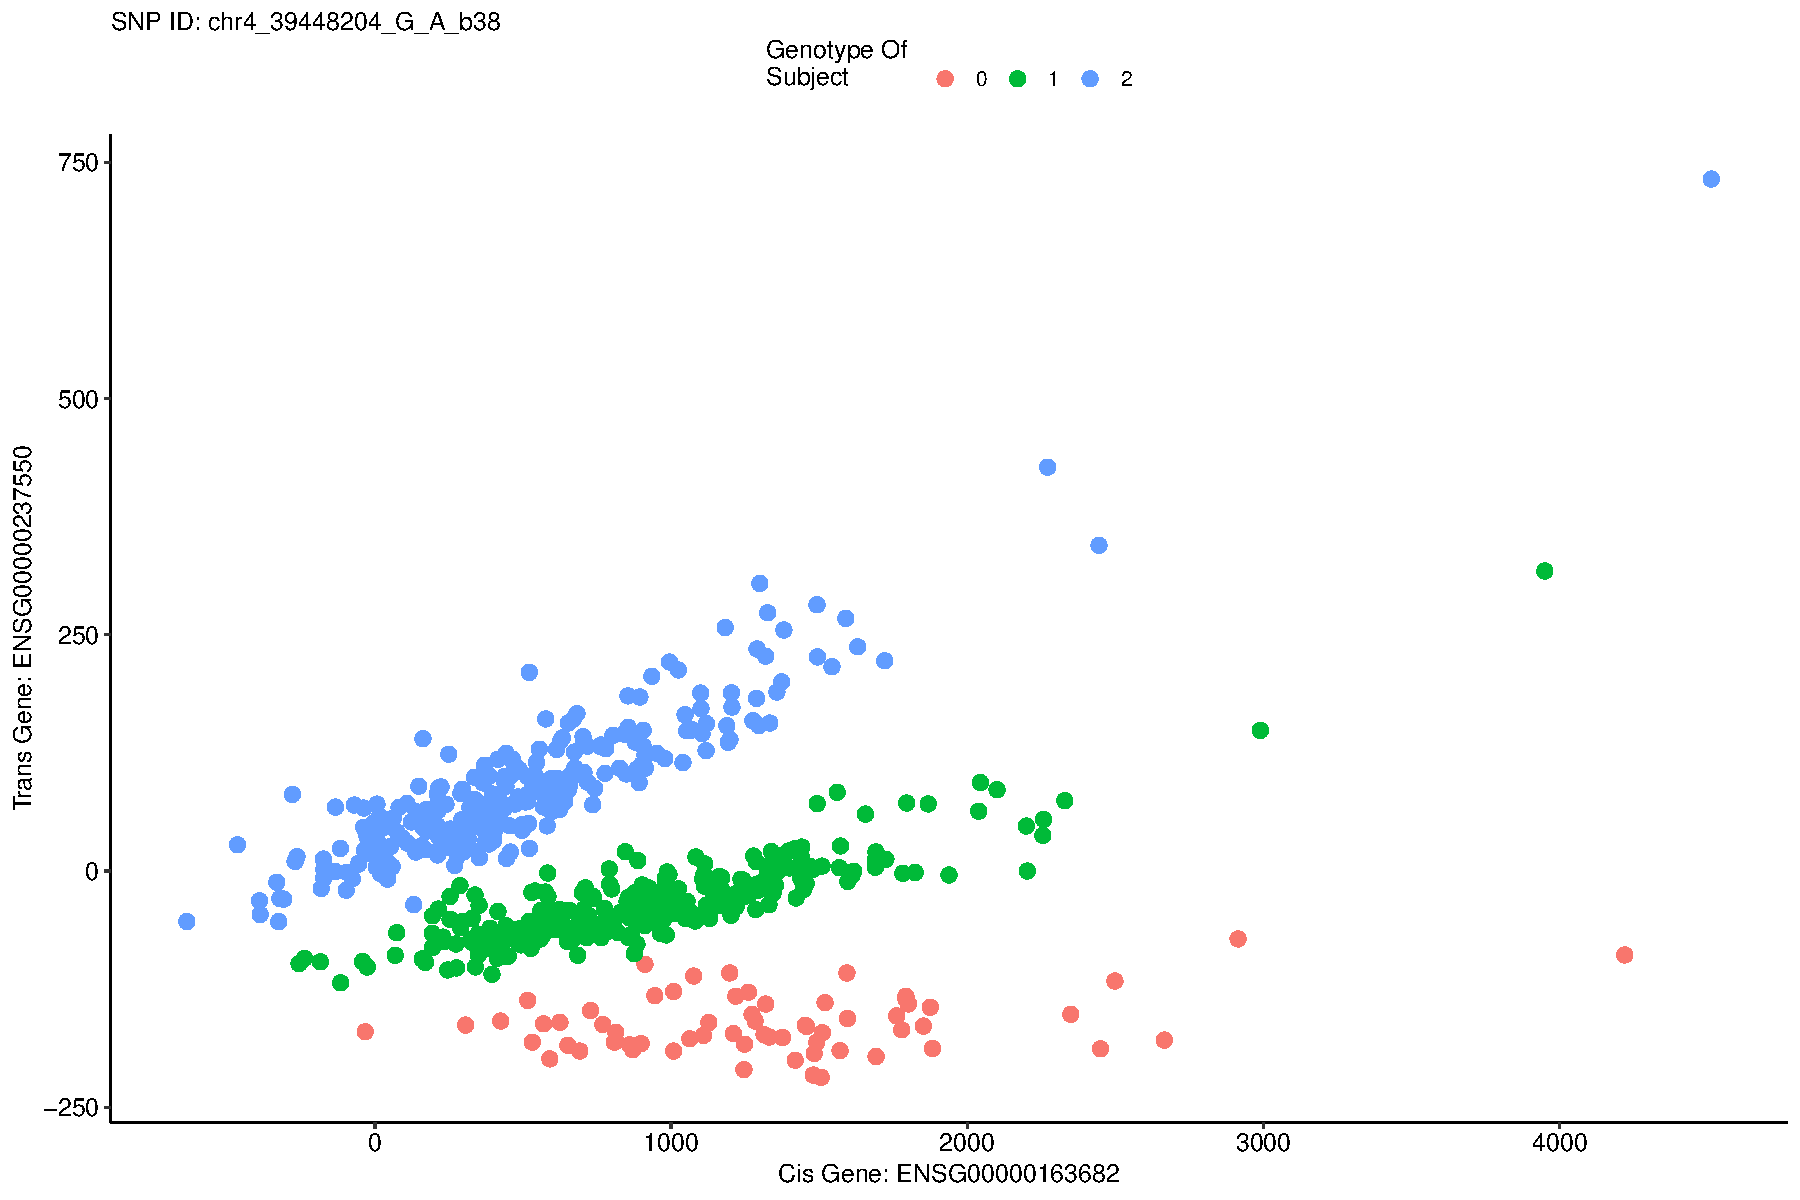
\includegraphics{12_15_2021_GMAC_plots_all_trios_files/figure-latex/unnamed-chunk-8-1.pdf}

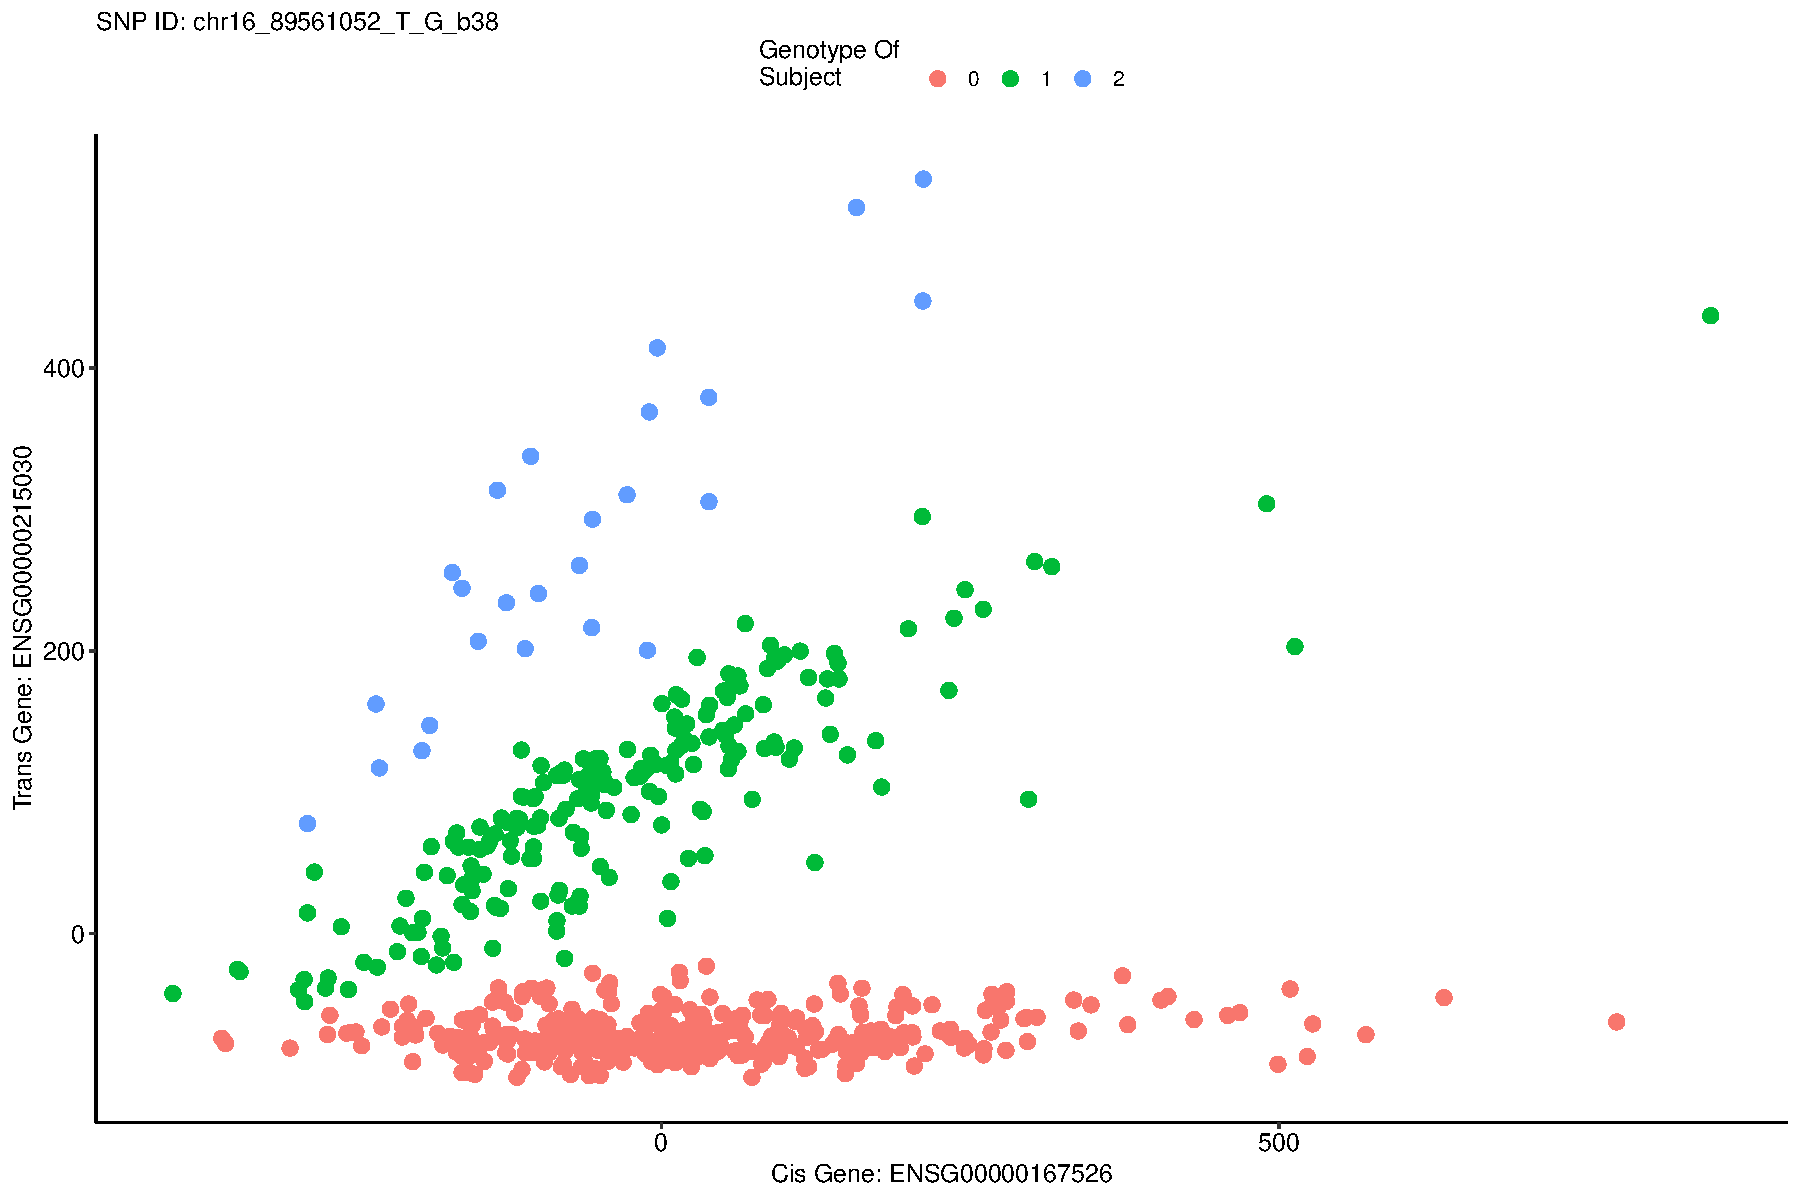
\includegraphics{12_15_2021_GMAC_plots_all_trios_files/figure-latex/unnamed-chunk-9-1.pdf}

\begin{figure}
\centering
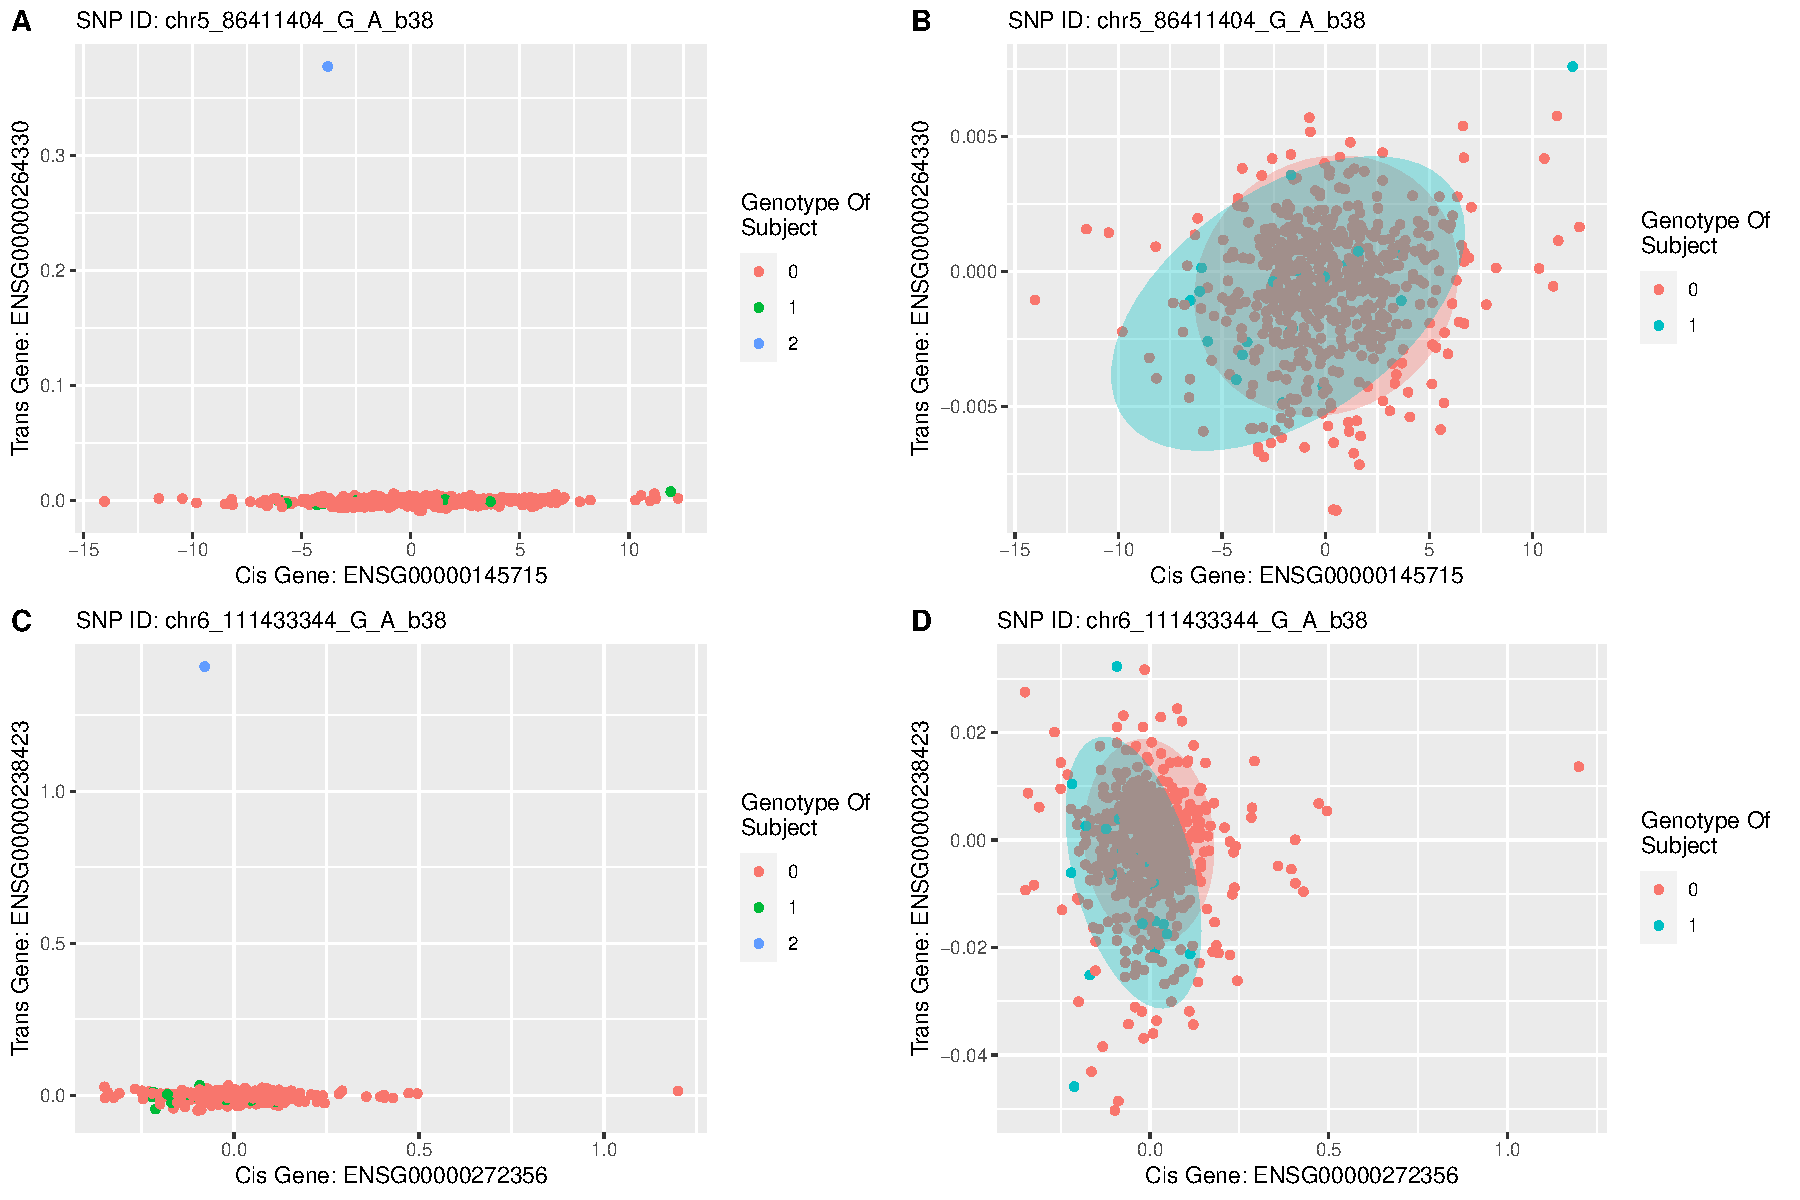
\includegraphics{12_15_2021_GMAC_plots_all_trios_files/figure-latex/unnamed-chunk-10-1.pdf}
\caption{\textbf{A} and \textbf{C}: Example scatter plots of trios from
subcutaneous adipose tissue and whole blood (respectively) with a rare
allele present in the sample: Note that 0 indicates individuals
homozygous for the reference allele, 1 indicates hetezygous individuals
and 2 indicates individuals who are homozygous for the alternative
(rare) allele. The apparent outlier represents a single individual in
the sample who was homozygous for the rare allele, and \textbf{B} and
\textbf{C} are the scatter plots with the point(s) for the
homozygous-alternative individuals removed and a confidence ellipse
calculated over the remaining homozygous-reference and heterzygous
individals.}
\end{figure}

\end{document}
